We now consider the \emph{modified modified greedy} algorithm~\ref{alg:mmgreedy}
\footnote{A paraphraze on the ``ultimate ultimate weapon'' from \cite{ninjago2017}}

\begin{algorithm}[H]
\label{alg:mmgreedy}

\SetKwInOut{Input}{input}
\SetKwInOut{Output}{output}

\Input{$U = \{e_1, \dots, e_n\}$, $f:2^U\to \mathbb{R}_+$, $c:U \to \mathbb{R}_+$}
\Output{$S \subseteq U$}

$S \leftarrow \text{greedy}(U, f, c)$
\\
\Return{$\arg\max\{S, \displaystyle{\arg\max_{e_1, e_2 \in U}}f(\{e_1, e_2\})\}$}
\caption{Modified Modified Greedy Algorithm}
\end{algorithm}

We now analyze the modified modified greedy algorithm.

Let $\epsilon > 0$ a constant to be determined latter on, and let $T$ be the output of 
the algorithm.

\begin{theorem}
$f(S) \geq 1 - e^{-(1/2 + \epsilon)}$
\end{theorem}

\def\eps{0.104}
\begin{proof}
We can assume that $f(\{e_1, e_2\}) \leq 1 - e^{-1/2 + \epsilon}$ 
for every $e_1, e_2 \in U$ or otherwise the proof holds.
Note, also, that if $|O \setminus T| \leq 2$ then $f(T) \geq 0.5$.
Thus we assume the algorithm drops at least three elements from $O$ during its running.
Let $x$ be the first element in $O$ that was dropped by the algorithm, 
and let $A$ be the set of elements chosen by the algorithm just before dropping $x$.
If $f(A) \geq 1 - e^{-(1/2 + \epsilon)}$ the theorem holds, 
otherwise denote $f(A) = 1 - e^{-(1/2 + \epsilon - \delta)}$.
We say that an element, $e$, is \emph{expensive} if $c(e) \ge 1/4 + \epsilon/2 - \delta/2$, 
otherwise it is \emph{cheap}.
Observe that $O$ contains at most two expensive elements, thus the algorithm drops 
at least one cheap element from $O$. 
Let $y$ be the first such element, and let $B$ be the set of elements chosen by the 
algorithm right after dropping $x$ and just before dropping $y$.
Also denote by $C$ the subset of cheap elements in $O$, 
i.e. $C = \{e \in O : c(e) < 1/4 + \epsilon/2 - \delta/2\}$.

We argue that the following inequalities hold:

\begin{align}
c(A) \leq 0.5 + \epsilon - \delta 
\\
c(x) > 0.5 -\epsilon + \delta
\\
c(C) \leq 0.5 + \epsilon - \delta
\\
f(C) \ge e^{-1/2 + \epsilon}
\\
c(B) \ge 1/4 - 3\epsilon/2 + 3\delta/2
\\
f(B|A) \ge \left[
e^{-(1/2 + \epsilon)}
- (1 - e^{-(1/2 + \epsilon - \delta)})
\right]
(1-e^{-\frac{1-6\epsilon+6\delta}{2+4\epsilon-4\delta}})
\\
f(T) \geq \max_\epsilon \min \{1 - e^{-(0.5 + \epsilon)}, \min_{\delta} f(A) + f(B|A)\}
\end{align}
\todo{explain the inequalities}.

Substituting $f(A) = 1 - e^{-(1/2 + \epsilon - \delta)}$ into the last inequality, 
using $f(B|A) \ge \left[
e^{-(1/2 + \epsilon)}
- (1 - e^{-(1/2 + \epsilon - \delta)})
\right]
(1-e^{-\frac{1-6\epsilon+6\delta}{2+4\epsilon-4\delta}})
$,
and setting (say) $\epsilon = \eps$ gives the desired result 
as can be seen in Figure~\ref{fig:mmgreedy}.

\end{proof}

\begin{figure}
\caption{
\label{fig:mmgreedy}
Modified Modified Greedy Approximation Ratio ($\epsilon = \eps$)
}
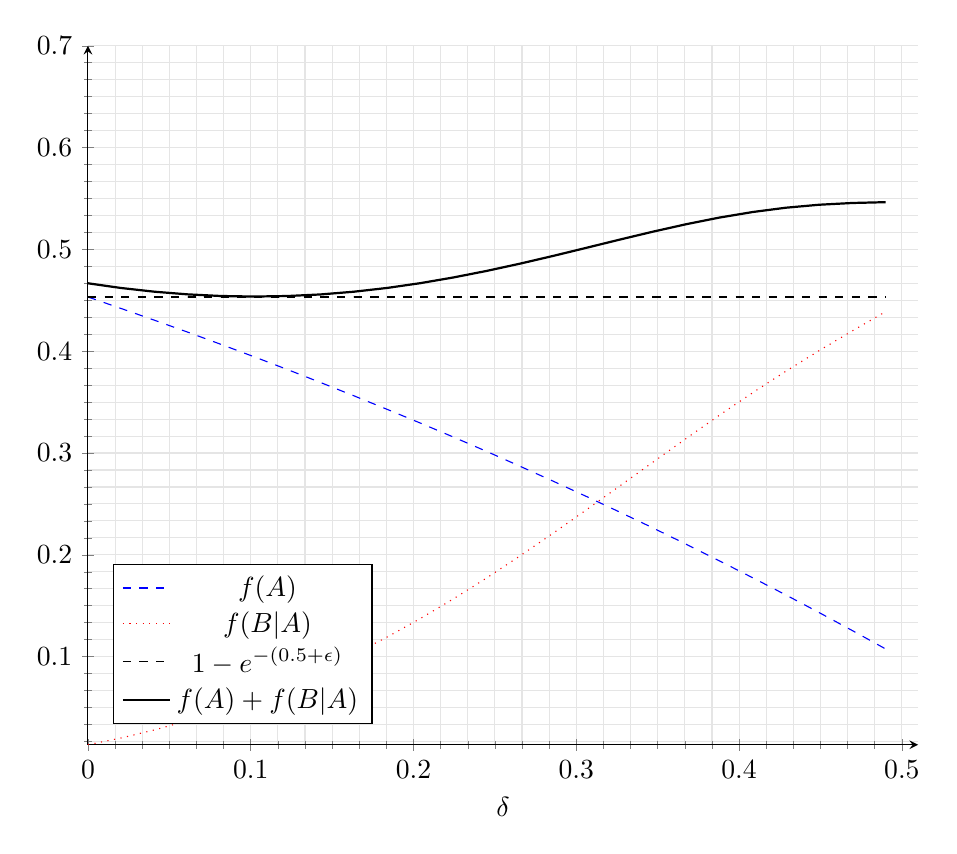
\begin{tikzpicture}
\begin{axis}[
	width=\textwidth
	,domain=0:0.49
	,ymax=.7
	,xmax=.51
	,xlabel=$\delta$
	,xtick distance=0.1
	,ytick distance=0.1
	,axis lines=left
	,grid=both
	,grid style={
		draw=gray!20
	}
	,minor tick num=5
	,legend pos=south west
	,legend entries={
		$f(A)$
		,$f(B|A)$
		,$1-e^{-(0.5 + \epsilon)}$
		,$f(A) + f(B|A)$
	}
]
  \addplot[blue, dashed, thin]{1-exp(-(0.5 + \eps -x))};
  \addplot[red, dotted, thin]{
  	(1 - exp(-(1 - 6 * \eps + 6 * x)/(2 + 4 * \eps - 4 * x)))
  	*
  	(exp(-(0.5 + \eps)) - 1 + exp(-(0.5 + \eps - x)))
  };
  \addplot[black, dashed]{
  	1-exp(-(0.5 + \eps))
  };
  \addplot[black, thick]{
  	1-exp(-(0.5 + \eps -x))
  	+
  	(1 - exp(-(1 - 6 * \eps + 6 * x)/(2 + 4 * \eps - 4 * x)))
  	*
  	(exp(-(0.5 + \eps)) - 1 + exp(-(0.5 + \eps - x)))
  };
\end{axis}
\end{tikzpicture}
\end{figure}

\paragraph{Upper Bound}
We show that the approximation ratio of the modified modified greedy algorithm is at most $0.5$.
To see this consider the following instance of the budgeted maximum coverage problem:
Let the elements be $X = \{x_1, \dots, x_{2n}\}$, 
and a collection of subsets over $X$, $\mathcal{S} = \{S_1, \dots, S_{n + 1}\} \cup \{S\}$,
where for each $1 \leq i \leq n + 1$, $S_i = \{x_i\}$, and $c(S_i) = 1$. 
Also, set $S = \{x_{n + 2}, \dots, x_{2n}\}$, and $c(S) = n$.
Finally, for each $x \in X$ set $w(x) = 1$ and set the budget for this instance to be $2n$.
One can verify that the modified modified algorithm will return a solution of value $n + 1$
While taking $S$ along with any other $n$ subsets yields a solution of value $2n - 1$.  



